Se utilizo un equipo estándar compuesto por un microscopio óptico acoplado a
una cámara digital, un capcacitor de placas paralelas y un generador eléctrico
que polarizaba positivamente la placa superior, como se muestra en la
\cref{fig:set-up}.
La distancia entre las placas del capacitor fue de \(d = \qty{5.00}{\milli m}\)
y la diferencia de potencial aplicada entre ellas varió en un rango de
\( U = \qty{100}{V} \) a \qty{300}{V}.

Se empleó aceite de silicona con una densidad de
\( \rho_{ac} = \qty{919.9}{kgm^{-3}} \), que se atomizó en pequeñas gotas
utilizando un atomizador controlado.
Las gotas fueron observadas bajo el microscopio mientras se desplazaban entre
las placas del capacitor.

\begin{figure}[htbp!]
    \centering
    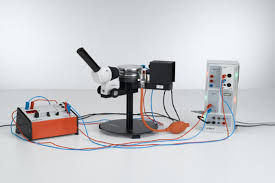
\includegraphics[width=0.8\linewidth]{./images/Montaje-Experimental.jpeg}
    \caption{Montaje experimental.}
    \label{fig:set-up}
\end{figure}

Para medir las posiciones de las gotas de aceite en intervalos de tiempo, el
microscopio utilizado cuenta con una escala de \qty{20}{\milli m}.
El desarrollo tradicional de la práctica requiere de registrar estas distancias
usando un cronómetro, en este caso los tiempos se miden con la linea del tiempo
del vídeo.

El software \emph{Tracker Video} fue utilizado para analizar los vídeos obtenidos.
Ajustando una escala en el software, se pudo determinar la posición de las gotas
cuadro por cuadro.
Los datos generados por \emph{Tracker} fueron exportados en archivos para su
posterior análisis.
En la \cref{fig:Tracker} se muestra la interfaz del software, mientas que en la
\cref{fig:drop-tracker} se observa el proceso de rastreo de posición de dos
gotas.

\begin{figure}[htbp!]
    \centering
    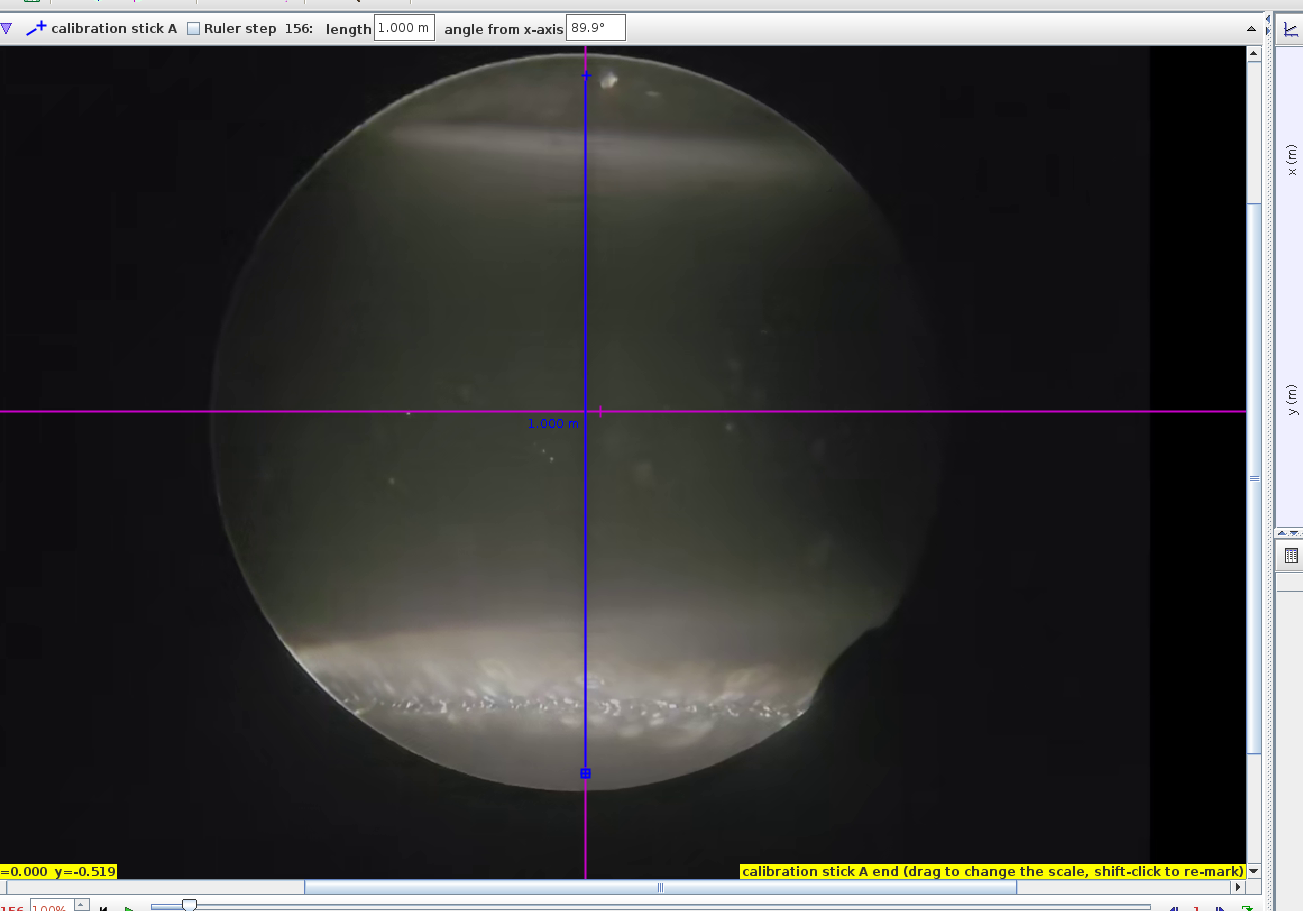
\includegraphics[width=0.8\linewidth]{./images/tracker-set-up.png}
    \caption{Interfaz de \emph{Tracker Video}.}
    \label{fig:Tracker}
\end{figure}

\begin{figure}
    \centering
    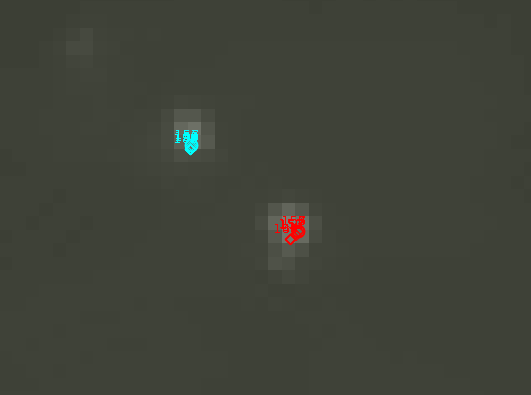
\includegraphics[width=0.8\linewidth]{./images/drop-tracker.png}
    \caption{Dos gotas vistas desde \emph{Tracker Video}.}
    \label{fig:drop-tracker}
\end{figure}

